\documentclass{article} % Define la clase del documento, en este caso, un artículo
\usepackage[letterpaper,margin=3cm]{geometry} % Configura el tamaño del papel y los márgenes del documento
\usepackage{graphicx} % Permite la inserción de imágenes
\usepackage[spanish]{babel}% Activar esta configuración para informes en español, ajusta el idioma del documento
\usepackage[usenames]{color} % Permite el uso de colores definidos por nombre en el documento
\usepackage{hyperref} % Habilita enlaces y referencias dentro del documento
\hypersetup{colorlinks=true, linkcolor = black, citecolor= black} % Configura el color de los enlaces y citas
\usepackage{booktabs} % Proporciona comandos para crear tablas de alta calidad
\usepackage{natbib} % Permite el uso de citas y referencias bibliográficas con diferentes estilos
\usepackage{tikz} % Permite la creación de gráficos y diagramas vectoriales directamente en LaTeX
\usepackage{float} % Para controlar la posición de los elementos flotantes, como imágenes, con la opción [H]
\usepackage{diagbox} % Permite crear celdas con líneas diagonales en tablas
\usepackage{listings} % Permite la inclusión y formateo de código fuente en el documento
\usepackage{xcolor} % Paquete para definir y usar colores en el documento
\usepackage{parskip} % Añade espacio entre párrafos en lugar de sangrías
\usepackage{fancyhdr} % Permite personalizar encabezados y pies de página
\usepackage{amsmath} % Proporciona una amplia variedad de entornos y comandos matemáticos

\pagestyle{fancy} % Usa el estilo fancyhdr
\fancyhf{} % Borra todos los encabezados y pies de página
\renewcommand{\headrulewidth}{0pt}
\renewcommand{\footrulewidth}{0pt} % Desactiva la línea horizontal predeterminada en el pie
\setlength{\headheight}{2cm} % Ajusta la altura del encabezado para hacer espacio para la línea
\fancyhead[L]{\raisebox{0.20cm}{\textbf{Métodos y Técnicas de Construcción}}} % Añade el texto en la parte izquierda del encabezado, subiéndolo ligeramente
\fancyhead[R]{\raisebox{0.1cm}{
\includegraphics[width=0.25\linewidth]{LOGO_UNIVERSIDAD.jpg}}} % Añade la imagen en la parte derecha del encabezado y súbela un poco
\fancyhead[C]{\rule{\textwidth}{0.6pt}} % Añade una línea horizontal superior centrada
\fancyfoot[C]{\rule{\textwidth}{0.6pt}} % Añade una línea horizontal en el pie de página centrada
\fancyfoot[R]{\raisebox{-1.5\baselineskip}{\thepage}} % Coloca el número de página a la derecha, con suficiente espacio debajo de la línea
\geometry{top=3cm, bottom=2.5cm} % Ajusta los márgenes superior e inferior

% Definición de colores al estilo Visual Studio Code
\definecolor{codegreen}{rgb}{0.25,0.49,0.48} % Comentarios
\definecolor{codegray}{rgb}{0.5,0.5,0.5} % Números y anotaciones
\definecolor{codepurple}{rgb}{0.58,0,0.82} % Palabras clave
\definecolor{backcolour}{rgb}{0.95,0.95,0.92} % Color de fondo

% Configuración del estilo de las celdas de código
\lstset{
    backgroundcolor=\color{backcolour},   % color de fondo; necesita que el paquete color o xcolor esté cargado
    commentstyle=\color{codegreen},       % estilo de comentarios
    keywordstyle=\color{codepurple},      % estilo de palabras clave
    numberstyle=\tiny\color{codegray},    % estilo de los números de línea
    stringstyle=\color{red},              % estilo de las cadenas de texto
    basicstyle=\ttfamily\small,           % estilo del texto básico
    breakatwhitespace=false,              % ajustes de líneas sólo en espacios en blanco
    breaklines=true,                      % ajustar las líneas si son muy largas
    captionpos=b,                         % posición de la leyenda (abajo)
    keepspaces=true,                      % preserva los espacios en el texto; útil si se usa monoespaciado
    numbers=left,                         % dónde poner los números de línea
    numbersep=5pt,                        % qué tan lejos están los números de línea del código
    showspaces=false,                     % mostrar espacios con subrayados particulares; reemplaza 'showstringspaces'
    showstringspaces=false,               % subrayar los espacios dentro de las cadenas solo
    showtabs=false,                       % mostrar tabulaciones en el código con subrayados particulares
    tabsize=2,                            % tamaños de tabulación a 2 espacios
    language=TeX,                         % lenguaje del código
    morecomment=[l]\#,                    % reconocer # como inicio de comentario en Python
    frame=single,                         % agregar un marco simple alrededor del código
    rulecolor=\color{black}               % color del marco
}

\begin{document}
%----------------------------------------------------------------------------------------
%   PORTADA
%Modificar desde aqui en adelante
%----------------------------------------------------------------------------------------
\begin{titlepage}%Inicio de la carátula, solo modificar los datos necesarios
\newcommand{\HRule}{\rule{\linewidth}{0.5mm}} 
\center 
%----------------------------------------------------------------------------------------
%	ENCABEZADO
%----------------------------------------------------------------------------------------

\includegraphics[width=10cm]{LOGO_UNIVERSIDAD.jpg}\\ % Si esta plantilla se copio correctamente, va a llevar la imagen del logo de la facultad.OBS: Es necesario incluir el paquete: graphicx
\vspace{3cm}
%----------------------------------------------------------------------------------------
%	SECCION DEL TITULO
%----------------------------------------------------------------------------------------
\HRule \\[0.4cm]
{ \huge \bfseries Tarea 2}\\[0.4cm] % Titulo del documento
{ \huge \bfseries Métodos y Técnicas de Construcción}\\[0.4cm] % Titulo del documento
\HRule \\[1.5cm]
 \vspace{5cm}
%----------------------------------------------------------------------------------------
%	SECCION DEL AUTOR
%----------------------------------------------------------------------------------------
\begin{flushright}
    { \textbf{Profesor:}\\
    Jose Tramon\\
    \vspace{0.2cm}
    \textbf{Alumnos:}\\
    Bernardo Caprile Canala-Echevarría\\
    Pedro Tomás Valenzuela Bejares\\
    \vspace{0.2cm}

}
\end{flushright}
\vspace{1cm}
%----------------------------------------------------------------------------------------
%	SECCION DE LA FECHA
%----------------------------------------------------------------------------------------
{\large \textbf{\today}}\\[2cm] % El comando \today coloca la fecha del dia, y esto se actualiza con cada compilacion, en caso de querer tener una fecha estatica, reemplazar el \today por la fecha deseada
\end{titlepage}
%----------------------------------------------------------------------------------------
%  INDICE
%----------------------------------------------------------------------------------------
\newpage
\tableofcontents
\thispagestyle{plain} % Deshabilita el encabezado en la página del índice
\thispagestyle{empty} % Deshabilita el número de página en la página del índice
\newpage

%Se puede agregar un indice de figuras si es nesesario
%\newpage
%\listoffigures 
%\thispagestyle{plain} % Deshabilita el encabezado en la página del índice %
%\thispagestyle{empty}
%\newpage
%----------------------------------------------------------------------------------------
%   ACÁ EMPIEZA EL INFORME
\setcounter{page}{1} % Reinicia el contador de páginas
%-------
\section{Introducción}
Este informe presenta la programación, valorización y seguimiento de avance de la construcción de un edificio de bodega. El objetivo es planificar las actividades necesarias, calcular los costos y preparar los pagos parciales para la obra.

Primero, se realizó la programación de actividades en MS Project, siguiendo un orden constructivo lógico, con estimaciones de duración y relaciones de precedencia entre tareas. Además, se identifica la ruta crítica y se establece un seguimiento del avance en diferentes etapas del proyecto.

Luego, se valorizó cada partida con precios actualizados a enero de 2024, considerando costos directos, gastos generales y un porcentaje de utilidad. También se preparan estados de pago al 15\% y 35\% de avance, ajustados por el IPC.

Este informe busca ofrecer una visión clara y estructurada del proceso de planificación y valorización, asegurando un seguimiento efectivo del proyecto y control de los costos.

\newpage
\section{Rendimientos}
En cada partida, dentro de las cuadrillas consideradas para los distintos trabajos, se incluyó tanto al personal de obra como a los operarios encargados de la operación de la maquinaria necesaria. Además, no se consideraron la excavación de escarpe ni la carpeta granular de rodadura, ya que estas no se utilizaban en esta etapa del proyecto.

\subsection{Movimiento de tierras, funadaciones y vialidad}
\subsubsection{Excavación a TCN Caminos y Bodegas}
Para estas dos partidas se consideró un rendimiento de 100 $\frac{m^3}{dia}$ por retroexcavadora, consiguiendo 1 y 26 días de trabajo respectivamente.

\subsection{Mejoramiento Fundaciones con integral natural}
Para esta partida se consideró un rendimiento de 28 $\frac{m^3}{dia}$ consiguiendo 35 y 14 días de trabajo respectivamente.

\subsubsection{Relleno Estructural bajo 2 y 6 pulgadas (entre Fundaciones hasta Subrasante)}
Para esta partida se consideró un rendimiento de 100 $\frac{m^3}{dia}$ por retroexcavadora, consiguiendo 2 y 3 días de trabajo.

\subsubsection{Formación y Construcción de Terraplenes (m³)}
Para esta partida se consideró un rendimiento de 90 $\frac{m^3}{hora}$ por cuadrilla de 4 a 6 personas. Con 2 cuadrillas se estima un tiempo total de 11 y 10 días.

\subsection{Preparación de la Subrasante}
Para esta partida se consideró un rendimiento de 400 $\frac{m^3}{dia}$ por retroexcavadora, consiguiendo 21 y 13 días de trabajo respectivamente.

\subsubsection{Base Granular CBR (m³)}
Para esta partida se consideró un rendimiento de 290 $\frac{m^3}{hora}$ por cuadrilla de 4 a 6 personas. Con 2 cuadrillas se estima un tiempo total de 4 días.


\subsubsection{Remoción de Pavimento Asfáltico (m²)}

Para esta partida se consideró un rendimiento de 70 $\frac{m^2}{hora}$ por cuadrilla de 3 a 5 personas, dependiendo de las herramientas y maquinaria empleada. Con 2 cuadrillas se estima un tiempo total de 1 día.

\subsubsection{Excavación en Terreno de Cualquier Naturaleza (TCN) (m³)}

Para esta partida se consideró un rendimiento de 22 $\frac{m^3}{hora}$ por cuadrilla de 4 a 6 personas. Con 5 cuadrillas se estima un tiempo total de 37 días.

\subsubsection{Hormigón}
Para esta partida se consideró un rendimiento de 28 y 21 $\frac{m^3}{hora}$, esto de la base que un camión mixer de $7m^3$ se demora aproximadamente 30 minutos en vaciarse. Por la gemometría del proyecto pueden estar vaciandose varios camiones al mismo tiempo, esto conlleva que en 1 hora se logren vaciar hasta 4 camiones mixer. Por ello, se consideraron los siguientes tiempos de trabajo:
\begin{itemize}
    \item Hormigón G-25 radier (malla acma C-92): 2 días
    \item Hormigón G-35 calles: 1 día
    \item Hormigón G-25 Fundaciones Zapatas Bodegas y Oficinas: 1 día
    \item Hormigón G-04 Emplantillado Fundaciones Galpones y Oficinas: 1 día
    \item Hormigón G-25 Vigas de Fundación Galpones y Oficinas: 1 día
    \item Hormigón G-25 Pedestales Galpones y Oficinas: 1 día
    \item Hormigón G-25 Muros Galpones y Oficinas: 1 día
\end{itemize}

\subsubsection{Acero para armaduras A63-42H}
Para esta partida se consideró un rendimiento de 1.12 $\frac{ton}{dia}$ por cuadrilla, para este trabajo se consideraron 3 cuadrillas, consiguiendo 13, 4, 7 y 8 días de trabajo.

\subsubsection{Demolición de Aceras ($m^2$)}

Para esta partida se consideró un rendimiento de 50 $\frac{m^2}{hora}$ por cuadrilla de 3 a 5 personas, dependiendo del equipo y condiciones del terreno. Con 2 cuadrillas se estima un tiempo total de 1 día.

\subsubsection{Remoción de Soleras (m)}

Para esta partida se consideró un rendimiento de 50 $\frac{m}{hora}$ por cuadrilla de 4 a 6 personas. Con 1 cuadrilla se estima un tiempo total de 1 día.

\subsubsection{Solera Tipo A (m)}

Para esta partida se consideró un rendimiento de 40 $\frac{m}{hora}$ por cuadrilla de 4 a 6 personas. Con 4 cuadrillas se estima un tiempo total de 9 días.

\subsection{Estructuras, revestiientos y terminaciones}

\subsubsection{Estructura Metálica Montado y Pintado (Kg)}
Para esta partida se consideró un rendimiento de 1.12 $\frac{ton}{dia}$ por cuadrilla, para este trabajo se consideraron 10 cuadrillas, consiguiendo 52 días de trabajo.

\subsubsection{Aislación (m²)}
Para esta partida se consideró un rendimiento de 60 $\frac{m^2}{dia}$ por cuadrilla de 3 a 5 personas. Con 8 cuadrillas se estima un tiempo total de 32 días.

\subsubsection{Divisiones interiores bodegas (m²)}
Para esta partida se consideró un rendimiento de 30 $\frac{m^2}{dia}$ por cuadrilla de 3 a 5 personas. Con 8 cuadrillas se estima un tiempo total de 32 días.

\subsubsection{Oficionas (m²)}
Para esta partida se consideró un rendimiento de 30 $\frac{m^2}{dia}$ por cuadrilla de 3 a 5 personas. Con 8 cuadrillas se estima un tiempo total de 10 días.

\subsubsection{Drenes (Cubodren) ($m^3$)}
Para esta partida se consideró un rendimiento de 10 $\frac{m^3}{hora}$ por cuadrilla de 4 a 6 personas. Con 5 cuadrillas se estima un tiempo total de 12 días.

\subsubsection{Portones Bodegas (N°)}
Para esta partida se consideró un rendimiento de 2 $\frac{unidad}{dia}$ por cuadrilla de 3 a 5 personas. Con 4 cuadrillas se estima un tiempo total de 6 día.

\subsubsection{Puertas exteriores (N°)}
Para esta partida se consideró un rendimiento de 2 $\frac{unidad}{dia}$ por cuadrilla de 3 a 5 personas. Con 2 cuadrillas se estima un tiempo total de 9 día.

\subsubsection{Muros cortinas, ventanas y puertas vidriadas (m²)}
Para esta partida se consideró un rendimiento de 25 $\frac{m^2}{dia}$ por cuadrilla de 3 a 5 personas. Con 8 cuadrillas se estima un tiempo total de 4 días.

\subsubsection{Porteria Acogida, bicicletero y barrera acceso (m²)}
Para esta partida se consideró un rendimiento de 10 $\frac{m^2}{dia}$ por cuadrilla de 3 a 5 personas. Con 2 cuadrillas se estima un tiempo total de 3 días.

\subsubsection{Sala eléctrica (m²)}
Para esta partida se consideró un rendimiento de 15 $\frac{m^2}{dia}$ por cuadrilla de 3 a 5 personas. Con 1 cuadrillas se estima un tiempo total de 3 días.

\subsubsection{Sala de agua potable (m²)}
Para esta partida se consideró un rendimiento de 15 $\frac{m^2}{dia}$ por cuadrilla de 3 a 5 personas. Con 1 cuadrillas se estima un tiempo total de 2 días.

\subsubsection{Sala residuos (m²)}
Para esta partida se consideró un rendimiento de 20 $\frac{m^2}{dia}$ por cuadrilla de 3 a 5 personas. Con 1 cuadrillas se estima un tiempo total de 2 días.

\subsubsection{Cierre Perimetral Acmaford (ml)}
Para esta partida se consideró un rendimiento de 30 $\frac{ml}{dia}$ por cuadrilla de 4 a 6 personas. Con 2 cuadrillas se estima un tiempo total de 4 días.

\subsubsection{Cierre Perimetral Bulldog (ml)}
Para esta partida se consideró un rendimiento de 15 $\frac{ml}{dia}$ por cuadrilla de 4 a 6 personas. Con 4 cuadrillas se estima un tiempo total de 7 días.

\newpage
\section{Valorización de Partidas}

A continuación se presenta un atabla con la valorizacion de las partidas de la obra. Esta informacion se ontuvo de fuentes de internet, como el portal de construccion ONDAC principalmente, entre otras. 

\begin{table}[H]
    \centering
    \begin{tabular}{|c|l|r|}
    \hline
    \textbf{ÍTEM} & \textbf{DESCRIPCIÓN} & \textbf{Precio total (CLP)} \\ \hline
    \multicolumn{3}{|c|}{\textbf{1. MOVIMIENTO DE TIERRAS, FUNDACIONES Y VIALIDAD}} \\ \hline
    1.1 & Excavación en TCN Caminos & 1,381,941 \\ \hline
    1.2 & Excavación en TCN Bodegas & 60,328,422 \\ \hline
    1.3 & Mejoramiento Fundaciones con integral natural (1,5 m.) & 143,606,922 \\ \hline
    1.4 & Mejoramiento Fundaciones con integral natural (0,5 m.) & 54,624,621 \\ \hline
    1.5 & Relleno Estructural bajo 2" (entre Fundaciones hasta Subrasante) & 40,779,294 \\ \hline
    1.6 & Relleno Estructural bajo 6" (entre Fundaciones hasta Subrasante) & 77,731,203 \\ \hline
    1.7 & Relleno Estructural bajo 2" Bodegas, Oficinas, VF & 63,029,982 \\ \hline
    1.8 & Terraplén caminos y áreas de servicio & 11,699,530 \\ \hline
    1.9 & Terraplén bajo radier bodegas & 10,016,500 \\ \hline
    1.10 & Preparación de la Subrasante Bodegas & 108,220,520 \\ \hline
    1.11 & Preparación de la Subrasante Caminos y Áreas de Servicio & 65,888,250 \\ \hline
    1.12 & Base Granular Caminos & 37,748,106 \\ \hline
    1.13 & Base Granular Bodegas & 61,578,981 \\ \hline
    1.14 & Hormigón G-25 radier (malla acma C-92) & 235,178,400 \\ \hline
    1.15 & Hormigón G-35 calles & 178,416,700 \\ \hline
    1.16 & Hormigón G-25 Fundaciones Zapatas Bodegas y Oficinas & 87,167,040 \\ \hline
    1.17 & Hormigón G-04 Emplantillado Fundaciones Galpones y Oficinas & 3,922,016 \\ \hline
    1.18 & Hormigón G-25 Vigas de Fundación Galpones y Oficinas & 11,758,920 \\ \hline
    1.19 & Hormigón G-25 Pedestales Galpones y Oficinas & 7,983,120 \\ \hline
    1.20 & Hormigón G-25 Muros Galpones y Oficinas & 42,073,200 \\ \hline
    1.21 & Enfierradura Fundaciones Zapatas Galpones y Oficinas & 50,117,600 \\ \hline
    1.22 & Enfierradura Vigas de Fundación Galpones y Oficinas & 12,119,900 \\ \hline
    1.23 & Enfierradura Pedestales Galpones y Oficinas & 24,798,800 \\ \hline
    1.24 & Enfierradura Muros Galpones y Oficinas & 28,168,400 \\ \hline
    1.25 & Demolición de Aceras & 675,000 \\ \hline
    1.26 & Remoción de Soleras & 273,000 \\ \hline
    1.27 & Solera Tipo A & 26,197,551 \\ \hline
    \multicolumn{3}{|c|}{\textbf{2. ESTRUCTURAS, REVESTIMIENTOS, CUBIERTAS Y TERMINACIONES}} \\ \hline
    2.1 & Estructura Metálica Montado y Pintado & 1,713,234,250 \\ \hline
    2.2 & Aislación & 83,382,000 \\ \hline
    2.3 & Divisiones Interiores Bodegas & 170,113,620 \\ \hline
    2.4 & Oficinas & 60,180,000 \\ \hline
    2.5 & Drenes (CuboDren) & 31,620,000 \\ \hline
    2.6 & Portones Bodegas & 20,300,000 \\ \hline
    2.7 & Puertas Exteriores & 8,700,000 \\ \hline
    2.8 & Muros Cortinas, Ventanas y Puertas Vidriadas & 127,371,850 \\ \hline
    2.9 & Portería Acogida, Bicicletero y Barrera Acceso & 20,800,000 \\ \hline
    2.10 & Sala Eléctrica & 9,600,000 \\ \hline
    2.11 & Sala Agua Potable & 5,700,000 \\ \hline
    2.12 & Sala Residuos & 6,300,000 \\ \hline
    2.13 & Cierre Perimetral Acmaford & 10,800,000 \\ \hline
    2.14 & Cierre Perimetral Bulldog & 19,800,000 \\ \hline
    \end{tabular}
    \caption{Precios totales para cada partida de la obra}
    \label{tabla-precios-totales}
\end{table}
    
Donde se obtuvo que el la obra costara:

\begin{table}[H]
    \centering
    \begin{tabular}{|l|r|}
    \hline
    \textbf{Descripción}      & \textbf{Valor (CLP)} \\ \hline
    Total                     & 3.733.385.639       \\ \hline
    Total + IVA               & 4.442.728.910       \\ \hline
    Utilidades de 3\%         & 133.281.867         \\ \hline
    Gastos Generales de 10\%  & 444.272.891         \\ \hline
    \end{tabular}
    \caption{Resumen de totales y utilidades.}
    \label{tabla-totales-utilidades}
\end{table}

Los gastos generales, se consideran los gastos extras de la obra, como lo son sueldos, limpieza, seguridad, entre otros. Estos gastos se consideran un 10\% del total de la obra. Por otro lado, las utilidades son el margen de ganancia que se le da a la empresa constructora, en este caso se considero un 3\% del total de la obra.

\newpage
\section{Precios Unitarios}

A continuacion se presenta la tabla de precios unitarios de ciertos elementos utilizados en las partidas de la obra.


\begin{table}[H]
    \centering
    \caption{Tabla de Precios Unitarios}
    \vspace{0.2cm}
    \label{tab:precios_unitarios}
    \resizebox{\textwidth}{!}{%
    \begin{tabular}{lllll}
    \toprule
                                           Descripción & Unidad &  Cantidad & Precio Unitario & Precio Total \\
    \midrule
    \textbf{Relleno Estructural bajo 6" (entre Fundaciones ...)} & \textbf{m3} & \textbf{1} & \textbf{} & \textbf{25.971} \\
                            Estabilizado c/ Flete 15km &     m3 &       1.2 &           18600 &        22320 \\
                        Placas compatadoras de 2000 kg &    dia &      0.16 &            5598 &          896 \\
                                             Jornalero &    dia &       0.2 &           13775 &         2755 \\
                         \textbf{Terraplén bajo radier bodegas} & \textbf{m3} & \textbf{1} & \textbf{} & \textbf{6.500} \\
                  Material para confeccionar terraplen &     m3 &       1.3 &            1000 &         1300 \\
                                       Agua industrial &     m3 &      0.06 &             680 &           41 \\
                                    Camion agua aljibe &    hor &    0.0074 &           22566 &          167 \\
                                  Motoniveladora 200HP &    hor &    0.0125 &           40000 &          500 \\
                             Rodillo compactador 10TON &    hor &      0.01 &           25000 &          250 \\
                                     Camion tolva 15m3 &    hor &    0.1257 &           28257 &         3552 \\
                                      Excavadora 20TON &    hor &    0.0125 &           30000 &          375 \\
                         Capataz moviemiento de tierra &    dia &  0.003986 &           29600 &          118 \\
                          Jornalera 40 horas semaneles &    dia &     0.016 &           12300 &          197 \\
    \textbf{Hormigón G-04 Emplantillado Fundaciones Galpon...} & \textbf{m3} & \textbf{1} & \textbf{} & \textbf{70.036} \\
                             Hormigon G-04 (provision) &     m3 &      1.05 &           47645 &        50028 \\
                                       Servicio bombeo &     m3 &         1 &            8240 &         8240 \\
                        Concretero colocacion hormigon &    dia &      0.49 &           23227 &        11382 \\
                                   Jornalero capachero &    dia &      0.02 &           19296 &          386 \\
                                   \textbf{Solera Tipo} A & \textbf{m} & \textbf{1} & \textbf{} & \textbf{21.247} \\
                              Solera tipo A 90x16x30cm &     mt &         1 &            7250 &         7250 \\
                 Hormigon H-20 estructuras (provision) &     m3 &      0.04 &           53702 &         2149 \\
                            Sika antisol bidon 4.5 lts &    bid &         1 &            9490 &         9490 \\
                                              Perdidas &      \% &         5 &               - &          582 \\
                                               Albañil &    dia &     0.042 &           28500 &         1197 \\
                                             Jornalero &    dia &     0.042 &           13775 &          579 \\
    \bottomrule
    \end{tabular}
    }
\end{table}


De esta tabla se puede observar que para todos los materiales se consideró el costo de la mano de obra y el costo de los materiales que se utilizan para la construcción de la obra. Esta información se obtuvo del Portal de Construcción ONDAC, donde se muestra todo lo necesasrio para poder llevar a cabo una unidad del elemento deseado.

Dentro de los criterios utilizados, se debe saber el tipo de actividad, quien la va a llevar a cabo y los materiales y herramientas que se utilizarán, es decir se deben considerar los recursos humanos y materiales que se utilizaran en la obra. Además se deben cosniderar los gastos generales, como lo son los trasportes y maquinaria utilizada. Finalmente algo a tener en consideracion en ciertos materiales es la perdida que puede ocurrir en el proceso de construcción, esta suele ser de un 5\% del total de material a utilizar.

\newpage

\section{Planeamiento de Actividades}

El proyecto tiene una duración total estimada de 282 días y se desarrolla de la siguiente forma: Comienza con movimientos de tierra, donde se realizan excavaciones tanto en caminos como en las áreas destinadas a bodegas. Estas actividades preparan el terreno para el mejoramiento de fundaciones, que incluye el uso de material integral natural para garantizar la estabilidad estructural. Posteriormente, se realizan las labores de relleno estructural, tanto bajo fundaciones como en áreas de bodegas y oficinas, preparando así el suelo para las etapas siguientes.

A continuación, se trabaja en la preparación de la subrasante y la colocación de la base granular, elementos esenciales para recibir los hormigones. Se ejecutan diversas partidas de hormigonado, como el emplantillado, el hormigón G-25 en zapatas, vigas y pedestales, y el hormigón G-35 para las calles, consolidando las estructuras fundamentales del proyecto. 

Una vez finalizadas estas bases, se da paso al montaje y pintado de la estructura metálica, seguido por actividades de aislación, muros cortinas, ventanas, y divisiones interiores en las bodegas y oficinas. Finalmente, se instalan elementos secundarios, como los portones de bodegas, las puertas exteriores, y los cierres perimetrales (ACMAFORD y Bulldog), completando así las terminaciones necesarias para concluir el proyecto de manera integral y dentro del plazo establecido.

\newpage

\section{Programación de Actividades}

A continuación, se presentan los avances al 5\%, 15\%, 25\%, 50\% y 75\% de la obra.

\begin{figure}[H]
    \centering
    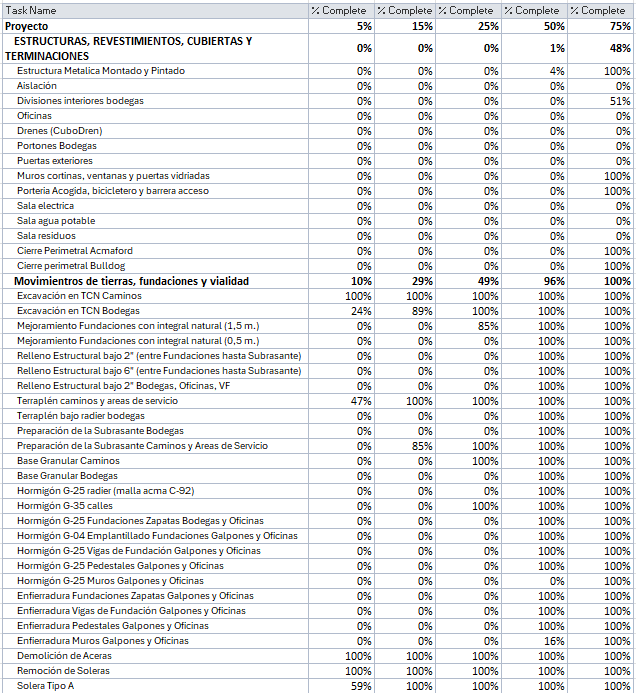
\includegraphics[width=1\linewidth]{GRAFICOS/P1A.png}
    \caption{Programación de actividades en Project}
    \label{fig:programacion}
\end{figure}

\newpage
\section{Estado de Pago}

El estado de pago es un documento que se utiliza para llevar un control de los pagos que se deben realizar en una obra, en este caso se presentan los estados de pago al 15\% y 35\% de avance de la obra. Esto es un pago que se realiza a los contratistas por el trabajo realizado en la obra, donde se ve un avance financiero de la obra, asi siguiendo los gastos y pagos de la obra. Esta se paga en base a ciertas partidas especificas que representan el avance en cierto porcentaje de la obra. Para esto se calculan los precios totales de la partida, incluyendo los gastos generales y utilidad. Luego se calcula el porcentaje de avance de la obra y se calcula el monto a pagar en base a este porcentaje.

\begin{table}[H]
    \centering
    \begin{tabular}{|c|c|}
    \hline
    \textbf{Mes} & \textbf{Valor} \\ \hline
    Enero       & 102.72         \\ \hline
    Octubre     & 105.56         \\ \hline
    \end{tabular}
    \caption{Valores del IPC por mes}
    \label{tabla:valores_mes}
\end{table}

Lo que deja una relación de 0.0269041 entre los valores de los meses, lo que indica que el valor de octubre es un 2.69\% mayor que el de enero. En este caso se utilizo el IPC de octubre ya que el de noviembre aun no esta dusponible.

Luego el monto reajustado queda para los avances de 15\% y 35\% respectivamente:

\begin{table}[H]
    \centering
    \begin{tabular}{|c|c|}
    \hline
    \textbf{Avance (\%)} & \textbf{Valor} \\ \hline
    15\%       & 15064211         \\ \hline
    35\%     & 20085615         \\ \hline
    \end{tabular}
    \caption{Reajustes segun el IPC}
    \label{tabla:reajuste}
\end{table}

Lo que queda en:

\begin{table}[H]
    \centering
    \begin{tabular}{|c|c|c|}
    \hline
    \textbf{Avance (\%)} & \textbf{Valor inicial}  &  \textbf{Valor reajustado}\\ \hline
    15\%       & 560007846 & 575072056      \\ \hline
    35\%     & 746677127 &  766762743     \\ \hline
    \end{tabular}
    \caption{Valores de los estados de pago} reajustados
    \label{tabla:reajustado}
\end{table}
    
\newpage
\section{Conclusión}

Este informe presentó un análisis de la programación, valorización y seguimiento del avance en la construcción de un edificio de bodega. La planificación de actividades permitió organizar las tareas de manera eficiente, optimizando recursos y garantizando el cumplimiento de los plazos establecidos. Además, se presentaron los avance de la obra al 5\%, 15\%, 25\%, 50\% y 75\% de la obra.

La estimación de rendimientos sirve para calcular tiempos y asignar cuadrillas y maquinaria de forma adecuada. Por otro lado, la valorización de partidas, mediante los precios unitarios, permitió proyectar el costo total del proyecto considerando materiales, mano de obra, maquinaria y posibles pérdidas.

Los estados de pago al 15 \% y 35 \% del avance simplifican el control financiero y lo dejan claro, asegurando la relación entre el progreso físico y los pagos realizados. Esto ayudó a mantener la transparencia y prever posibles ajustes en el presupuesto.

\newpage
\section{Referencias}
\nocite{*}
\bibliographystyle{plain}
\bibliography{referencias.bib}  

\end{document}